\chapter[Réionisation et masse des halos à z=0]{Lien entre les instants de réionisation des galaxies et la masse de leurs halo à l'époque actuelle}
\label{sec:z0}

\section{Le projet Cosmic Dawn}
\label{sec:CODAEMMA}

Toutes les simulations présentées dans les précédant chapitres avaient une taille de $\left( 8\cdot h^{-1} \mathrm{cMpc} \right)^3$.
Ce volume présente l'avantage de pouvoir réaliser un grand nombre de simulations facilement sans que cela ne soit trop coûteux en temps de calcul.
Mais il est admis que cette taille est trop faible pour étudier la réionisation dans son ensemble et que le panel de densités présentes dans ces simulations est restreint.
D'un coté les zones sous-denses sont sous représentées  (voir eg \cite{iliev_simulating_2006}) et de l'autre, nous avons vu en section \ref{sec:photonbudget} que le budget de photon n'est pas convergé dans ces volumes, et qu'il manque une partie des plus grosses galaxies ($M>10^{11}M_\odot$), ayant une formation stellaire importante.
Les séries de simulations utilisées dans les chapitres précédents ont pour vocation de calibrer et d'améliorer notre interprétation d'une simulation plus ambitieuse, "CoDa I AMR", que je vais présenter dans ce chapitre ainsi que les premiers résultats obtenus.
Dans cette partie nous utiliserons cette simulation pour obtenir de l'information sur l'histoire d'ionisation des galaxies actuelles.
Le lien entre l'\ac{EoR} et la période actuelle est réalisé en utilisant une seconde simulation, que je présenterai, ainsi que la façon dont le lien est réalisé.

%Cette partie repose sur une lettre qui s'inscrit dans une stratégie de travail a long terme.
%Ces résultats utilise deux simulations pour faire le lien entre la période de réionisation et l’époque actuelle.
%Je vais présenter les deux simulations utilisées et la façon dont le lien entre les deux est fait.
%xCette étude montre que les halos les plus massifs a z=0 sont réionisé plus tôt que le reste de l'Univers.

%Lettre donc partie courte.
%Objectif connaitre le Z reio des halo en fonction de leur masse.
%Sur grosse simu donc beaucoup de stats
%\subsection{Présentation de la simulation CODA II EMMA}

\subsection{Présentation du projet}

Le projet \ac{CoDa} a pour objectif l’étude la réionisation du Groupe Local. %, et de comprendre si il s'est fait réionisé par l'extérieur ou si il s'est réionisé de manière autonome.
Pour se faire, un contexte cosmologique suffisamment large est nécessaire pour modéliser l'influence des grandes structures proches comme Virgo ou Fornax par exemple.
Les conditions initiales ont été générées par la collaboration \ac{CLUES} \citep{2010arXiv1005.2687G}, avec pour objectif de retrouver dans la simulation, des structures ayant des caractéristiques proches de ce qui est observé dans l'univers local à $z=0$.
On cherchera par exemple à obtenir un couple Andromède - Voie Lacté avec des masses, distances et vitesses relative en accord avec les contraintes actuelles.
La figure \ref{fig:ortho} présente une visualisation de la simulation CoDa I - AMR, réalisée dans le cadre de ce projet.

\begin{figure}
        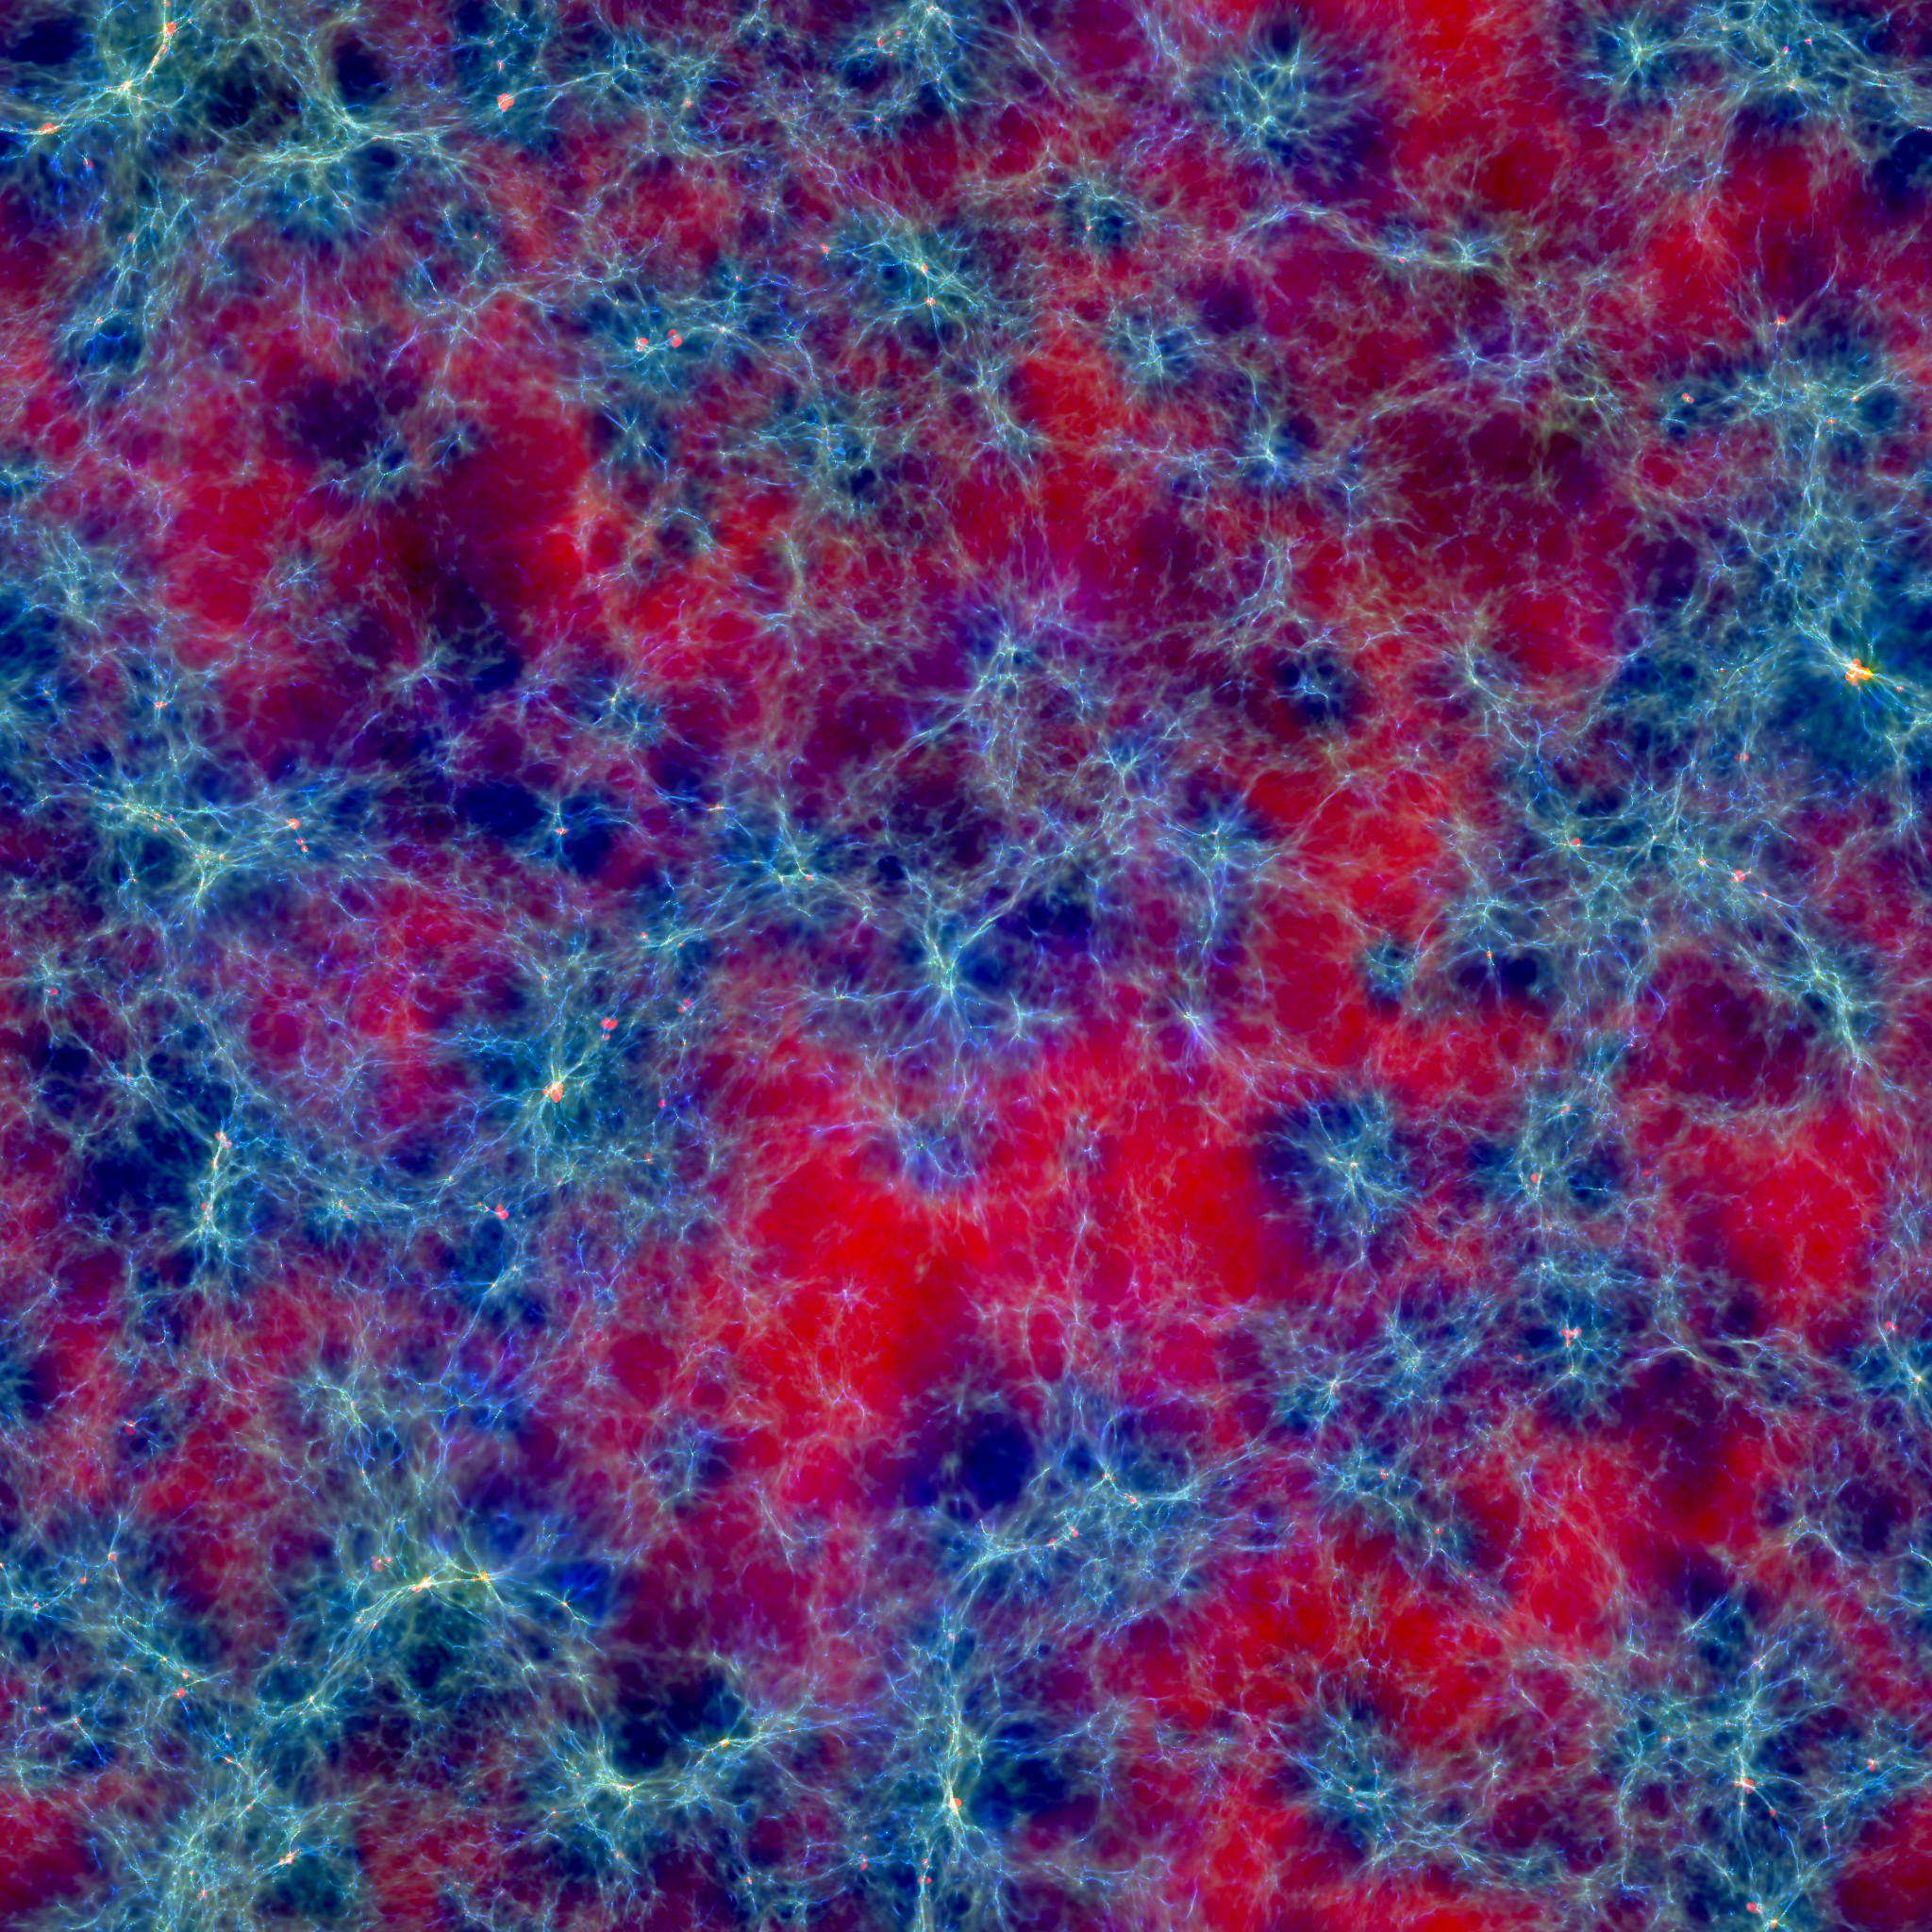
\includegraphics[width=.95\textwidth]{img/04/rgb-compose.jpeg} 
        \caption[Projection orthogonale]{Projection orthogonale de la simulation CoDa I - AMR sur une matrice $2048^2$.
        La projection correspond à la moyenne sur une tranche de 8/h cMpc d'épaisseur. 
        La composition RGB est réalisée avec dans l'ordre la température, la densité de gaz et la densité de gaz ionisé.
		Les vaste zones rouges correspondent aux vides qui ont reçut du rayonnement plus tard et n'ont pas encore eu le temps de refroidir par détente adiabatique.  
        }
 		\label{fig:ortho}
\end{figure}


\subsection{Conditions initiales}
\label{sec:ICCODA}
Les conditions initiales utilisées ici sont une version basse résolution de celles utilisées par la simulation \ac{CoDa} I \citep{ocvirk_cosmic_2015}.
%Cette simulation a été réalisé avec le code RAMSES CUDATON, %TODO ref
%considère un volume de $\left( 64/h \mathrm{cMpc} \right)^3$ et est échantillonné par $4096^3$ élements de résolutions (particules de matière noire et cellules de grille).
%Dans le cas de l'étude présentée ici, cette résolution a été dégradée en $2048^3$
Dans le cas de l'étude présentée ici, la simulation \ac{CoDa} I AMR considère un volume de $\left( 64/h \mathrm{cMpc} \right)^3$ et est échantillonné par $2048^3$ éléments de résolutions (particules de matière noire et cellules de grille), ce qui mène à une résolution en masse $3.4 \cdot 10^6 M_\odot$ et une résolution spatiale de 46 ckpc sur la grille de base, permettant d'explorer une gamme de masse de halos comprise entre $10^8 M_\odot$ et $10^{13}M_\odot$.
%La simulation \ac{CoDa} I dispose d'un niveau de résolution supérieur sur la grille de base, mais la perte de ce niveau de résolution supplémentaire est compensé par l'utilisation de l'\ac{AMR} de EMMA, permettant d’augmenter la résolution spatiale au détriment de la résolution en masse.
La résolution adaptative est bloquée à 500 pc, menant à l'ajout de trois niveaux de raffinements et permettant de gagner un facteur 4 en résolution spatiale par rapport à la simulation  \ac{CoDa} I.
L'objectif est de faire, dans un avenir proche, une comparaison directe entre les deux versions de cette simulation. % (CoDa I RAMSES CUDATON vs CoDa I AMR).

%différences avec CODA I RAMSES CUDATON et future comparaisons
%8x moins résolue en masse 
%Mais mieux résolue en dx

\subsection{Présentation des simulations}
\label{sec:presCODA}

A partir de ces conditions initiales plusieurs simulations ont été réalisées.

La première est une simulation \ac{RHD} entièrement couplée et réalisée avec EMMA.
Elle est focalisée sur l'\ac{EoR} et s’arrête donc à redshift $z=6$, une fois l'Univers réionisé.
Cette simulation a été exécutée sur le calculateur TITAN (voir section \ref{sec:titan}) et a utilisée 32768 cœurs \ac{CPU} et 4096 \ac{GPU}.
Les travaux présentés dans la section \ref{sec:etoiles} ont permis de calibrer correctement cette simulation.
Les comparaisons aux contraintes observationnelles de la \ac{SFH} cosmique, de l'évolution de le fraction ionisée et de l'épaisseur optique Thomson sont présentées sur la figure \ref{fig:presCODAEMMA}, on mesure une bonne concordance.
%Pour ces grandeurs la concordance est bonne.

Comme il est actuellement techniquement impossible de réaliser un simulation présentant des caractéristiques similaires à la simulation \ac{CoDa} I \ac{AMR} en l'exécutant jusqu’à redshift $z=0$, une seconde simulation à été réalisée.
Celle-ci est une simulation N-corps pur, ne considérant que la matière noire et a été réalisée avec le code Gadget \citep{springel_cosmological_2005} jusqu'à redshift $z=0$.
Elle a pour objectif de suivre l'évolution des structures jusqu'à aujourd'hui.

La simulation EMMA a pour but d'obtenir une représentation complète de l'époque de réionisation via sa carte de redshifts de réionisation.
L'implémentation du calcul de cette carte à la volée (voir section \ref{sec:zmapcompute}) a permis d'obtenir une excellente résolution temporelle.
Cependant, des difficultés de gestion mémoire ont menés à arrêter le calcul de cette carte à la volée à partir de redshift $z=8$.
Après ce redshift, la carte a été obtenue à l'aide des sorties disques, plus espacées en temps.
Malgré cet incident, la résolution temporelle est au pire de $1,4$ Myrs à redshift $z=6$, ce qui est inférieur au temps de vie d'une étoile, et reste donc acceptable.


\begin{figure}
        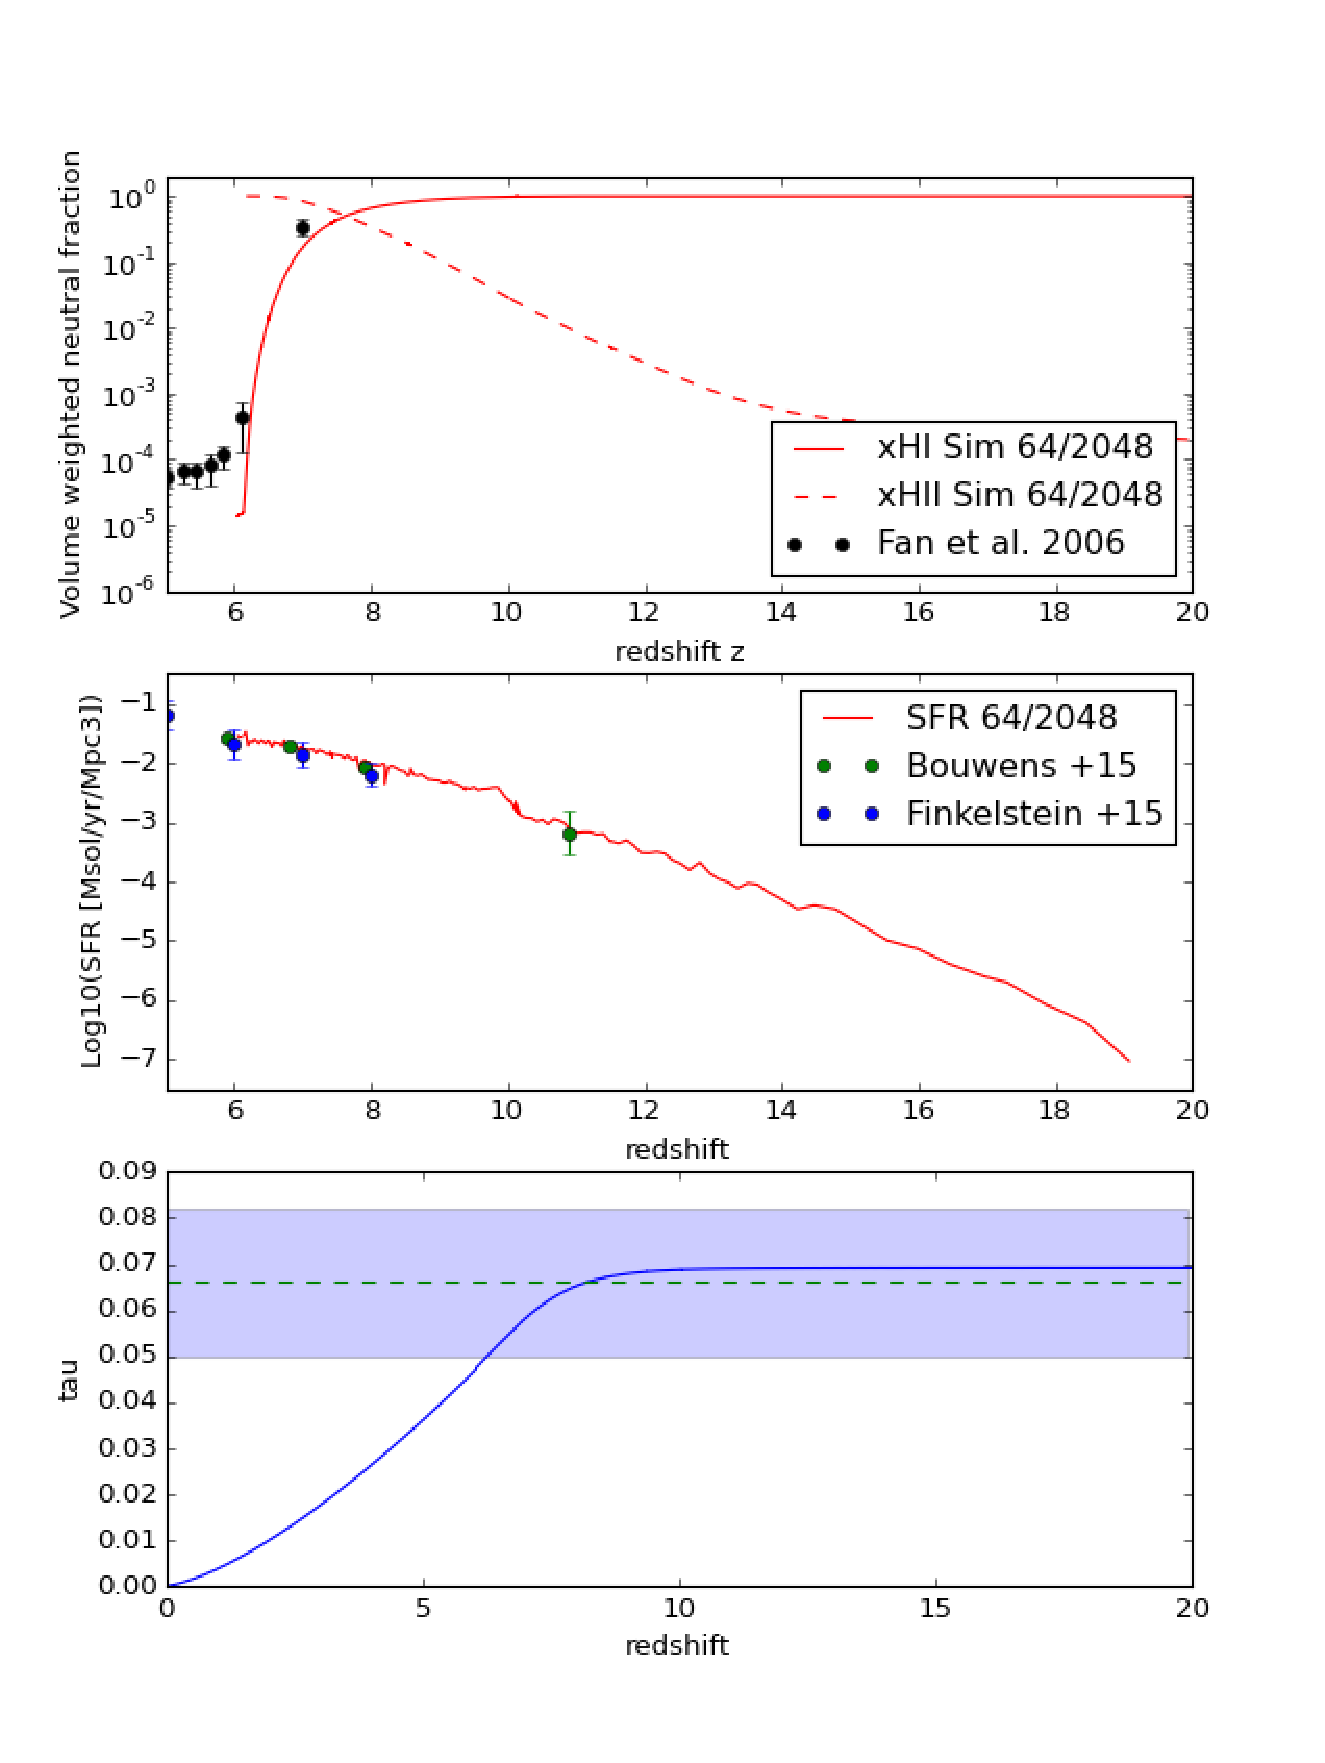
\includegraphics[width=.95\linewidth]{img/05/x_sfr_tau.pdf} 
%		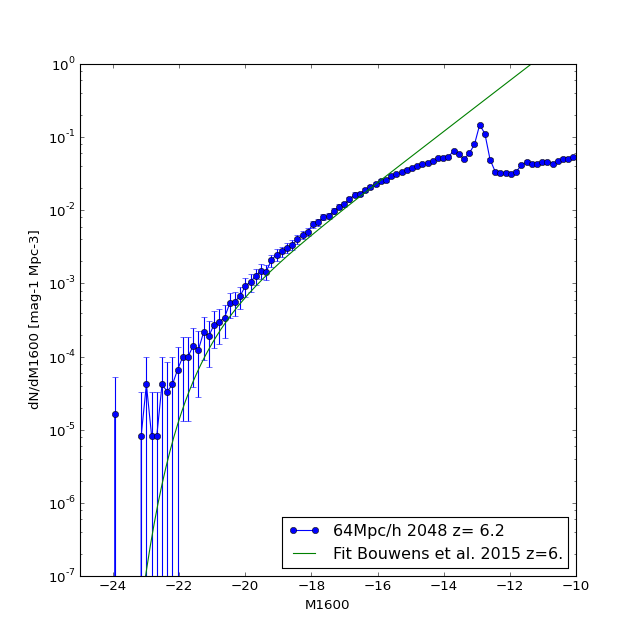
\includegraphics[width=.95\linewidth]{img/05/LFCODA .png}
        \caption[Contraintes CoDa I AMR]{ Variables globales de la simulation \ac{CoDa} I \ac{AMR} réalisée avec EMMA.
        Panneau supérieur : histoire d'ionisation
		Panneau central : SFH cosmique.
        Panneau inférieur : épaisseur optique Thomson.
        La simulation présente un bon accord avec les contraintes observationnelles.
		\label{fig:presCODAEMMA}}
\end{figure}


\section{Détermination des redshifts de réionisation des halos à redshift z=0}

L'objectif est ici de déterminer l'histoire d'ionisation des galaxies à $z=0$ et de leur environnement.
Cette histoire peut par exemple avoir eu un impact sur les propriétés des populations de satellites observées aujourd'hui.
Il à été démontré que le timing de réionisation influe sur la formation stellaire des galaxies de faibles masses ($M<10^9M_\odot$) \citep{ocvirk_reionization_2014}, une réionisation précoce aura tendance à photo-évaporer plus facilement les petites galaxies.
Également \citep{2015ApJ...800...34G} ont montré que la réionisation peut avoir un impact sur la distribution spatiale de satellites observées aujourd'hui.

%Nous cherchons ici à quantifier l'hétérogénéité du processus.
%, et ainsi estimer l'impact de la réionisation sur leurs propriétés observées.

La méthode consiste créer le lien entre les deux simulations réalisées en utilisant la carte de redshifts de réionisation d'un coté et la distribution de matière noire de l'autre.
%L'idée est ici que le l'influence gravitationnelle des baryons est négligeable par rapport à celle de la matière noire.
%Ce qui fait que l'introduction de l'hydrodynamique du gaz dans la simulation EMMA n'a pas significativement impacté la distribution de matière à redshift $z=6$ et que cette distribution est comparable à celle mesurée dans la simulation Gadget.
%Cette hypothèse est vérifiée, dans une certaine mesure, 
La population de halos trouvée dans la simulation Gadget est superposée à la carte de redshifts de réionisation obtenue avec la simulation EMMA sur la figure \ref{fig:zmapcomp}..
Les halos se trouvent effectivement aux centres des régions ionisées.
Il est donc à priori possible de lier la réionisation mesurée dans la simulation EMMA à l'évolution des structures mesurée dans la simulation Gadget.
%La méthode de projection n'est pas unique est principalement deux pistes ont été explorées.
Il existe plusieurs façon de faire ce type de lien, et principalement deux pistes ont été explorées.
%La figure \ref{fig:methodes} est une représentation graphique de ces deux méthodes.

%En considérant que le couplage entre la matière noire et les baryons et faible, la comparaison entre les catalogues de halos des deux simulations pris a la même époque peux être réalisé directement.

\begin{figure}
		\centering
        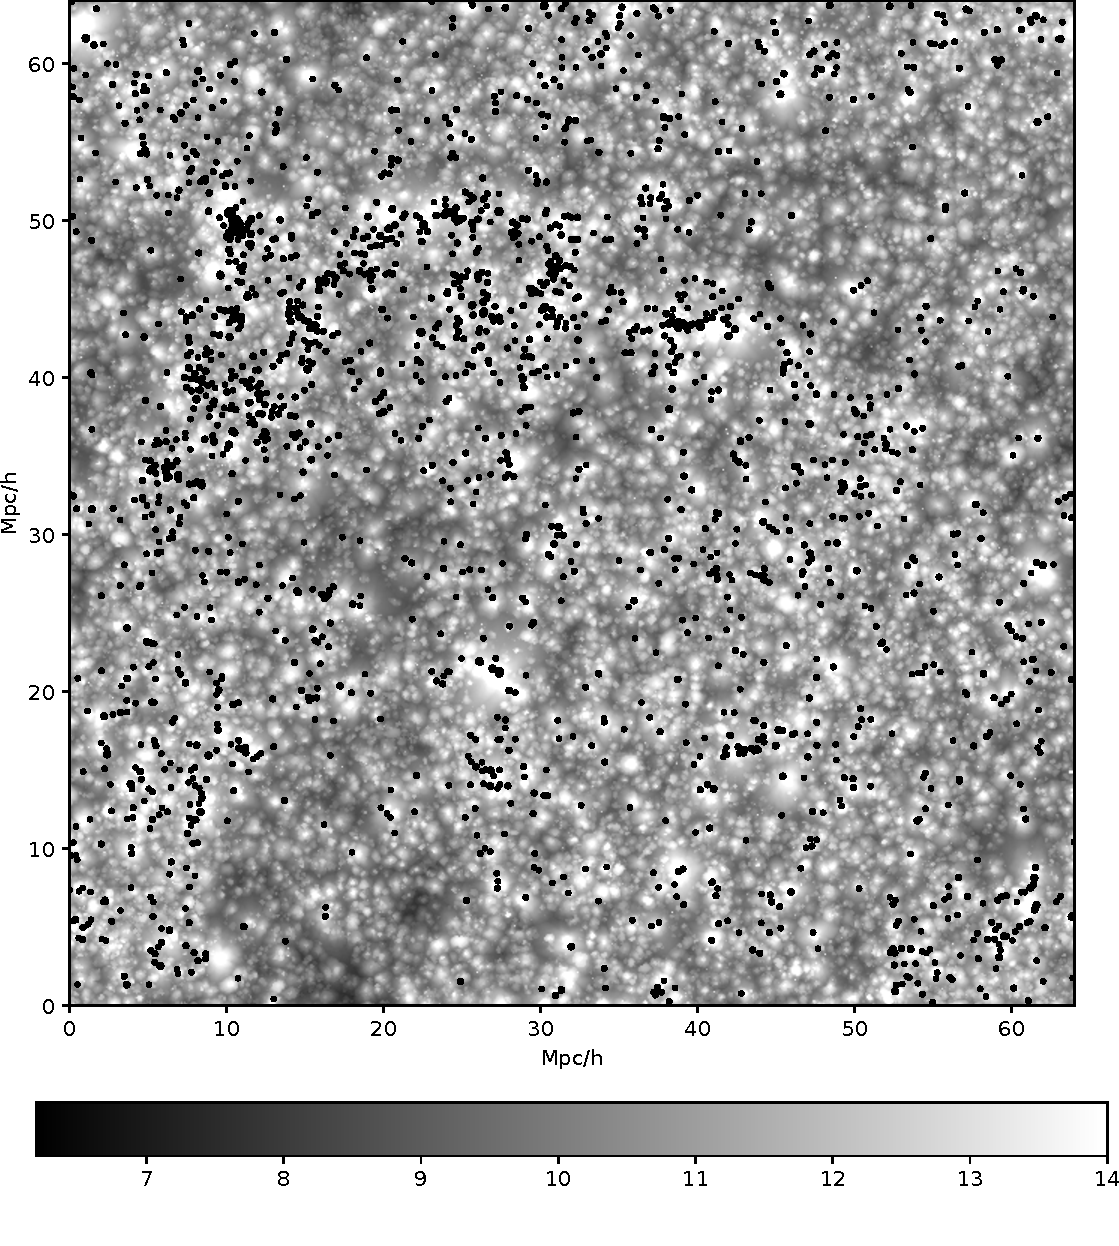
\includegraphics[width=.95\linewidth]{img/05/maphaloh.pdf} 
        \caption[Carte de redshift et halos]{Carte de redshift de réionisation calculée par la simulation \ac{RHD} EMMA et positions des halos à redsihft z=0 calculées avec la simulation, matière noire pure Gadget.
        La concordance des deux simulations est correcte, les halos de trouvent aux centres des régions ionisées.
		\label{fig:zmapcomp}}
\end{figure}


%\begin{figure}
%		\centering
%        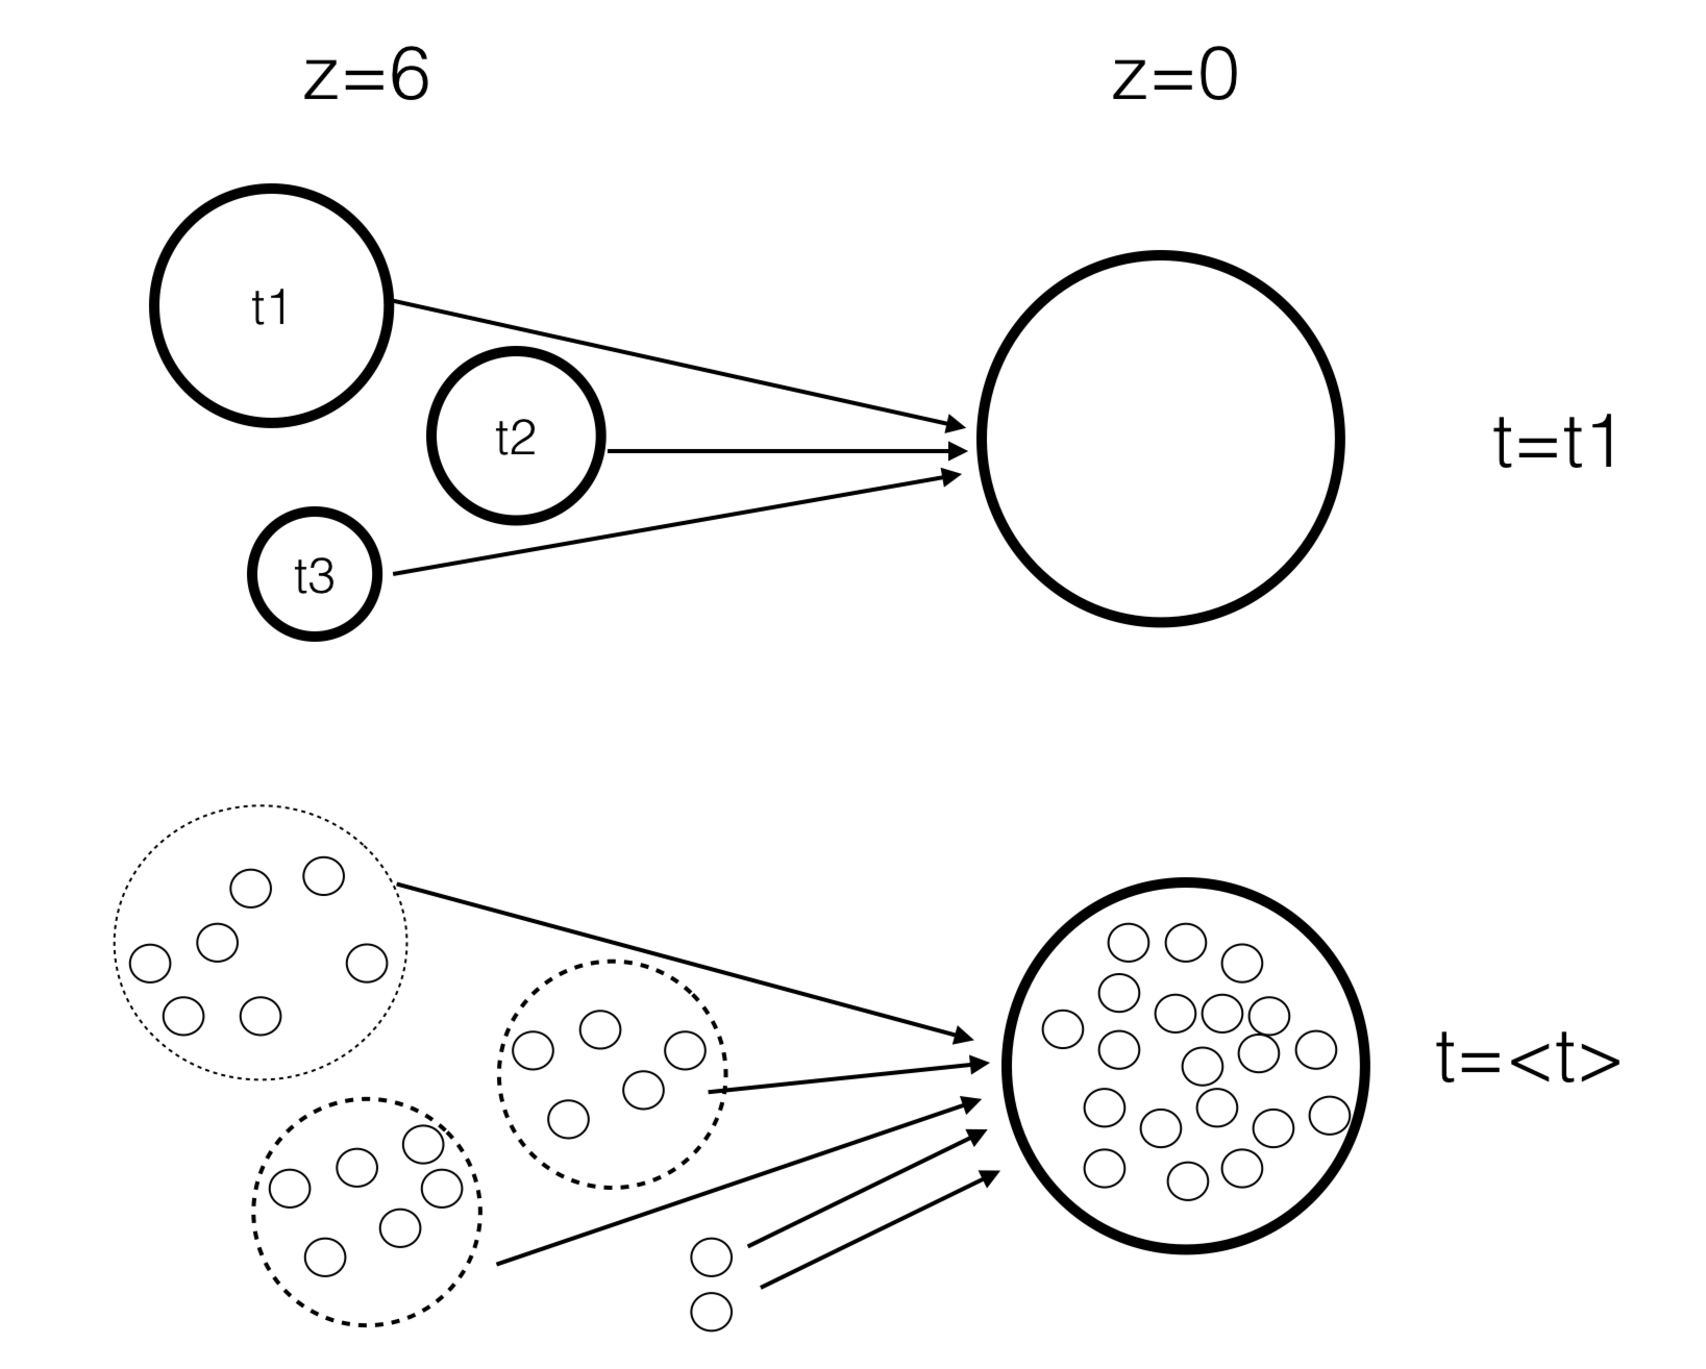
\includegraphics[width=.95\linewidth]{img/05/method.pdf} 
%        \caption[Methodes]{Représentation des deux méthodes d'assignation de redshift de réionisation aux halos de la simulation gadget.
%        Méthode "merger tree" en haut, méthode "particule" en bas
%		\label{fig:methodes}}
%\end{figure}


\subsection{Méthode "Merger Tree"}
La première méthode se base sur un un arbre de fusion (merger tree) des halos, généré sur la simulation Gadget.
%présentation du merger tree
Il permet de suivre les histoires de formation des halos de redshift $z=100$ jusqu'à nos jours.
En considérant un halo donné à redshift $z=0$, il est possible de déterminer, grâce à l'arbre de fusion, la position du centre de masse de tous ses halos progéniteurs à redshift $z>6$.
%A chacune de ses position est ensuite associée un instant d'ionisation en utilisant la carte de redshift de réionisation.
%A partir de l'arbre de fusion, et
En partant de redshift $z=20$, on cherche le premier instant où le progéniteur le plus massif appartient à une cellule ionisée.
%Le redshift de réionisation associé au halo, et celui du progéniteur le plus massif à redshift $z=6$.
Cette méthode impose que le halo en question ait au moins un progéniteur à redshift $z>6$ et considère donc en priorité les halos les plus massifs à $z=0$.

\subsection{Méthode "Particules"}
La seconde technique utilise les particules de matière noire.
En ayant la liste de toutes les particules de matière noire d'un halo donné à redshift $z=0$, il est possible de retrouver leurs positions dans toutes les sorties.
De la même manière que précédemment, on défini le redshift de réionisation comme le premier instant où une particule appartient à une cellule ionisée.
Un redshift de réionisation est donc obtenu pour chaque particule du halo et la valeur finale du redshift de réionisation associée au halo est la moyenne de cette liste.
Cette méthode permet de sonder les halos moins massifs qui n'avaient pas de progéniteurs aux redshifts $z>6$.

\section{Résultats}

%Les résultats qui vont être présentés dans cette section représente une étude préliminaire globale de la simulation.
%Évidemment, les simulations \ac{CoDa} ont encore énormément de potentiel scientifique à exploiter.

\subsection{Instants d'ionisation des halos}

Nous avons associé un redshift de réionisation pour chaque halos à redshift $z=0$ de la simulation Gadget.
%Il est donc possible de déterminer en fonction de la classe de masse du halo à $z=0$ un redshift de réionisation, 
%Pour le méthode ainsi qu'une durée de réionisation.
Le panneau supérieur de la figure \ref{fig:CODA_t} représente l'instant d'ionisation, en fonction de la masse du halo à $z=0$ pour les deux méthodes d'association.
Les traits représentent la valeur médiane dans l'intervalle de masses, les régions grisées représentent les limites de distributions à 5\% et 95\%.
La ligne noire horizontale représente l'instant où la fraction ionisée moyenne de la totalité du volume devient supérieure à 50\%, seuil également utilisé dans le calcul de la carte de redshift de réionisation (voir section \ref{sec:zmapcompute}).

On mesure ici que les halos les plus massifs reionisent avant la moyenne du volume, indépendamment de la méthode, et ce d'autant plus qu'ils sont massifs.
Ceci suggère un réionisation interne, puisque les halos massifs sont déjà peuplés d'étoiles à ces redshift, et ce d'autant plus qu'il sont massifs.
Cependant la méthode du progéniteur a tendance à réioniser plus tôt, car elle se concentre sur les halos déjà formés à haut redshift, et possédant donc des sources de rayonnement interne à cette époque.
Par ailleurs, même si ceux ci ne possèdent pas d'étoiles, il se trouvent généralement dans des régions denses ayant une probabilité importante de contenir des halos émettant déjà du rayonnement.
A l'inverse la méthode des particules a tendance à retarder la réionisation des halos. 
Dans ce cas des particules n'appartenant pas à des halos à $z>6$ se trouvent prises en considération.
Ces particules sont alors situées dans l'\ac{IGM}, elles sont plus représentatives du volume et ont donc des instants de réionisation plus tardifs.

La gamme de masses $M <10^{11} h^{-1}M_\odot$, a tendance à réioniser en même temps que la moyenne, cependant la médiane est légèrement en retard car nombre de ces halos ont peu, voir pas d'étoile, et semblent être soumis à une influence externe.
Il faut donc du temps pour que le rayonnement les atteigne.
De plus, ils sont plus denses que l'\ac{IGM} et vont donc nécessiter plus de temps pour ioniser leur masse supplémentaire.


%Pour les halos les moins massifs ($M<10^9 h^{-1}M_\odot$), la méthode du progéniteur tend à diminuer, car la probabilité qu'un halo de $10^8 h^{-1} M_\odot$ ait un progéniteur à $z>6$ est relativement faible.
%Visuellement, ceux qui en ont effectivement un semble localisé dans les régions denses, ayant donc des redshift de réionisation plus important.

%Pour les deux méthodes; les halos de masse $M \approx 10^{10} M_\odot$ à z=0 présentent un instant similaire, et semble présenté une certaine convergence.
%Ces halos présentent de masses pouvant être représentatif des halos ayant des masses de $M \approx 10^9 M_\odot$ à $z=6$, 

\begin{figure}
		\centering
        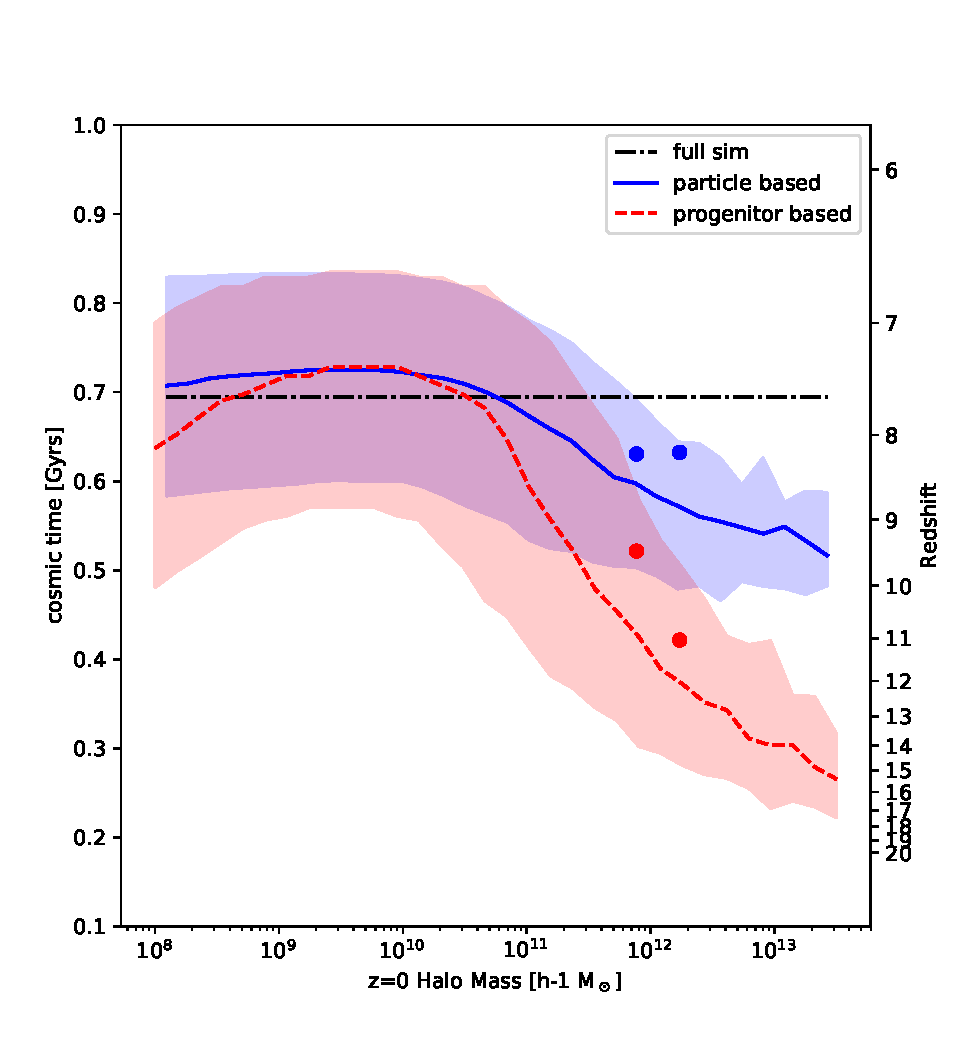
\includegraphics[height=.45\textheight]{img/05/track_treion_LG.pdf}
        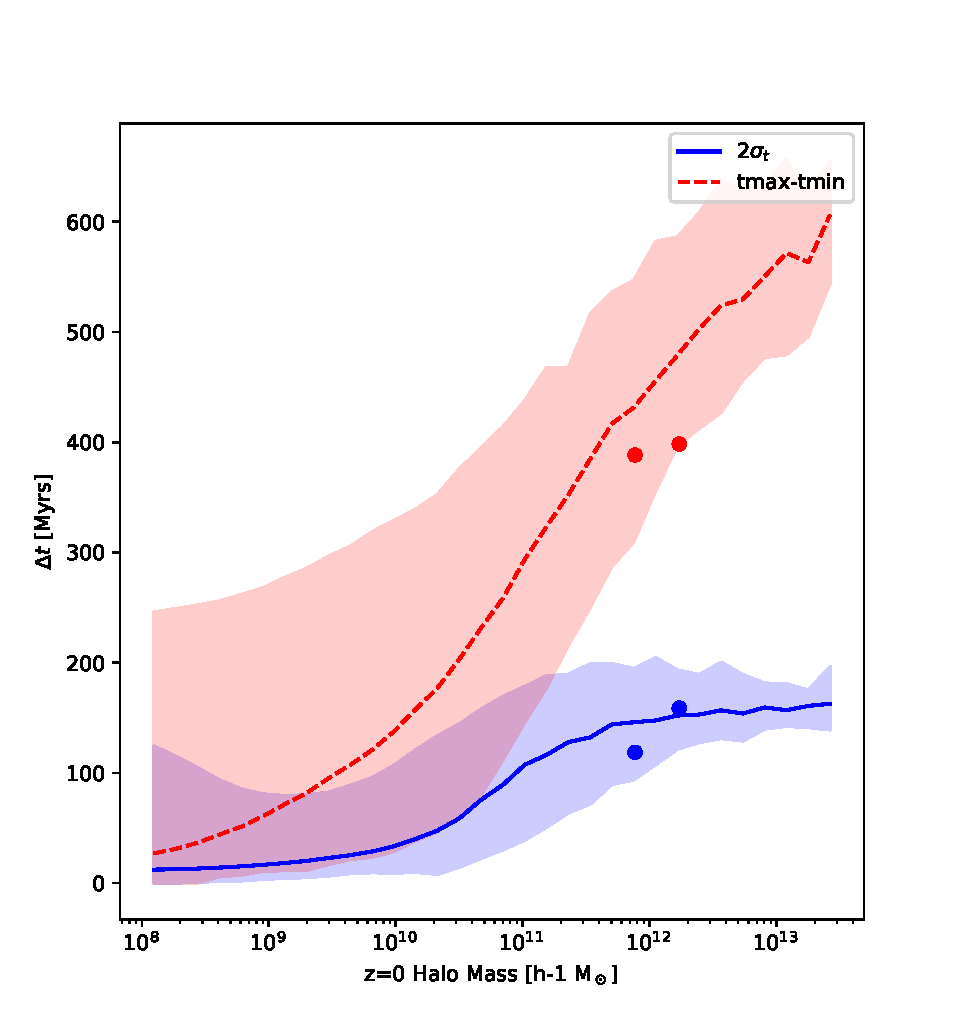
\includegraphics[height=.45\textheight]{img/05/track_dt_2sig_LG.pdf} 
        \caption[Instant et durée de réionisation]{Instant (panneau supérieur) et durée (panneau inférieur) de réionisation en fonction de la masse des halos à redshift $z=0$, pour les deux méthodes d'association. 
        La ligne horizontale représente $z\approx7.8$ l'instant ou la volume total atteint 50\% d'ionisation.
        Les points représentent le couple Voie Lacté - Andromède.
		\label{fig:CODA_t}}
\end{figure}


\subsection{Durée d'ionisation des halos}

Nous cherchons dans cette section à déterminer la durée de réionisation des halos en fonction de leurs masses.
Nous utilisons la méthode des particules pour associer une liste de redshifts de réionisation à chaque halos.
La détermination de la durée peut être réalisée de différentes manières, voici les deux méthodes utilisées:
\begin{itemize}
\item Dans un premier cas, la durée de réionisation a été associée à la différence entre le premier et le dernier instant où une particule a été ionisée au sein du halo.
\item Dans le second cas, pour chaque halos, on calcul la RMS de la distribution des redshifts, et la durée associée correspond à $\Delta t_{2\sigma} =  ( \langle t_{part} \rangle + \sigma) - ( \langle t_{part} \rangle - \sigma)$.
\end{itemize}

Le second panneau de la figure \ref{fig:CODA_t} présente les durées nécessaires à la réionisation des halos en fonction de leurs masses.
Comme attendu, la méthode de la RMS limite les durées extrêmes et en moyenne la durée est toujours plus basse que dans la méthode des maximas.

Dans les deux méthodes, les halos les plus massifs ont une durée de réionisation plus importante, les halos les plus massifs ont une étendue spatiale plus importante, il faut donc plus de temps au rayonnement pour les parcourir.
De plus ces halos ont plus de matière et nécessitent donc plus de photons pour être réionisés.
Avec la méthode des maximas, le halo le plus massif a, une durée de réionisation de 600 Myrs, durée comparable à la durée de l'\ac{EoR} dans la simulation.
Ce halo contient de la matière provenant d'une vaste diversité d’environnements. % et met en évidence 
Avec la méthode de la RMS, cette durée est réduite à 120 Myrs.

Les halos de masses $M \approx 10^{12} h^{-1}M_\odot$ similaires à MW ou M31 ont des durées comprises entre 60 et 120 Myrs, ce qui est comparable aux durées mesurées par \cite{ocvirk_reionization_2014} dans des volumes plus petits et centré sur le Groupe Local par exemple.
Dans leur modèle une durée de l'ordre de 120 Myrs est typique d'une scénario de réionisation interne, alors que les durées de 60 Myrs sont typiques d'une réionisation externe.

Les plus petits halos ont une durée qui tend vers zéro car leur taille est proche de celle de la résolution de la carte de redshifts et peuvent être inscrit dans une cellule.
Ce type de comportement suggère un réionisation par un front externe.

On remarquera que les durées de réionisation des halos $M > 10^{11} h^{-1}M_\odot$ sont comparables à la dispersion des instants de réionisation et donc un modèle de réionisation hétérogène doit inclure les effets d'une réionisation non instantanée.



%\begin{figure}
%		\centering
%    %    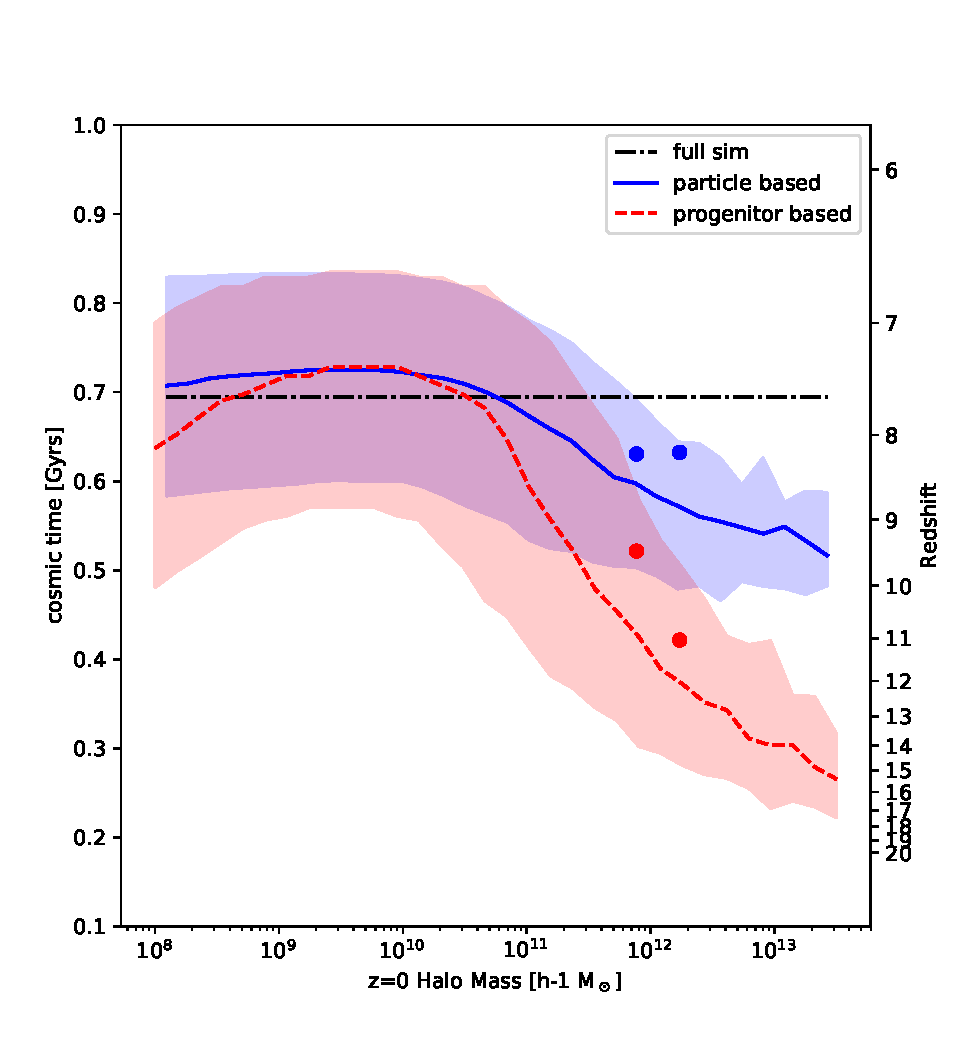
\includegraphics[width=.95\linewidth]{img/05/track_treion_LG.pdf}
%        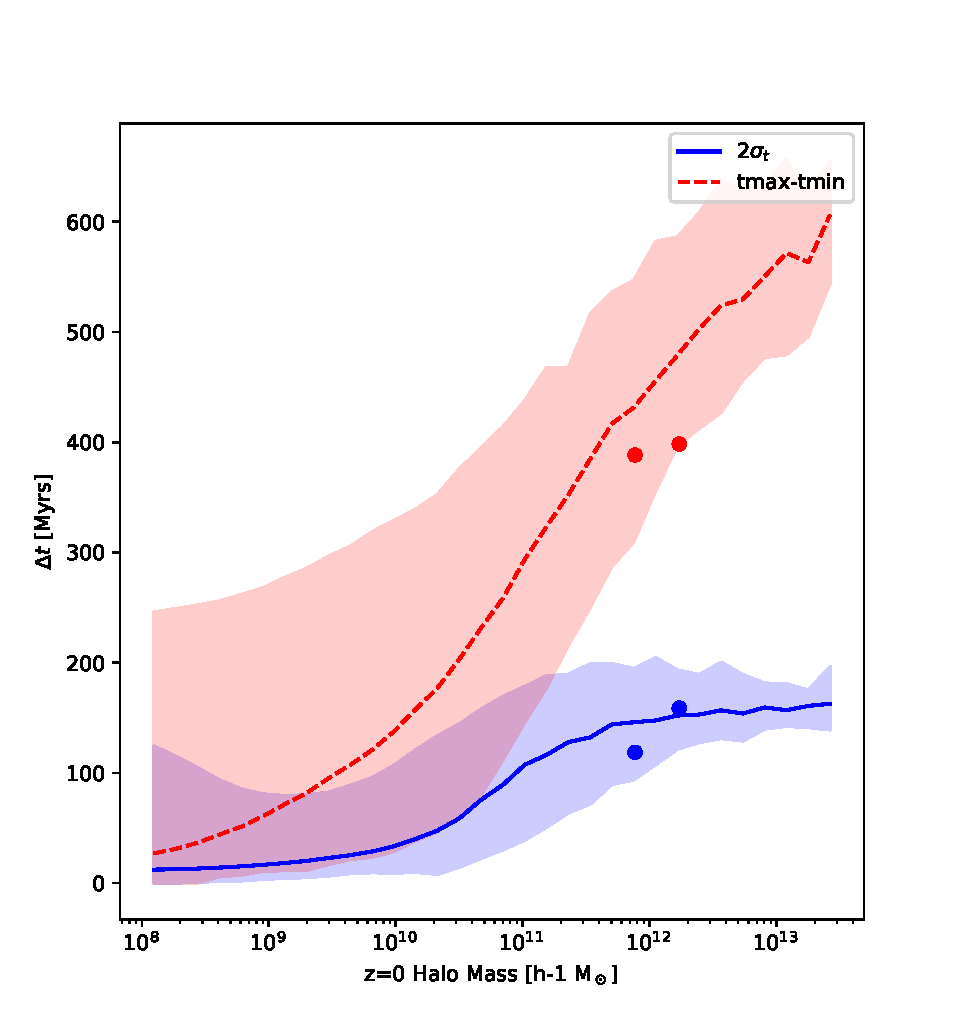
\includegraphics[width=.95\linewidth]{img/05/track_dt_2sig_LG.pdf} 
%        \caption[t et dt reio]{
%		\label{fig:CODA_t}}
%\end{figure}

%\subsection{Étude d’environnement}
%
%Dans le cas d'un environnement dense, le milieu aura tendance a produire plus de sources de photons mais sera en même temps plus dur à réioniser car plus d'atomes sont présent et le taux de recombinaison y est plus élevé. %TODO ref
%%dans la section  Nous avons abordé le problème de la compétition 
%Dans le but d'explorer la balance entre ces deux effets, le volume total de la simulation a été découpé en huit parties égales.
%Du fait de la variance cosmique, chacune de ces sous-parties dispose de sa propre densité moyenne.
%La figure \ref{fig:CODA_environnement} présent la comparaison des durées de réionisation obtenues avec la méthode 2$\sigma$, sur l'ensemble du volume, dans le sous volume le moins dense et dans le sous volume le plus dense.
%Nous mesurons, que le sous-volume le moins dense a une durée d'ionisation comparable à celle du volume total.
%Nous mesurons également qu'un environnement plus dense mène en moyenne à une durée de réionisation plus courte.%, et donc la production de photon supérieure compense les effets 
%
%\begin{figure}
%		\centering
%		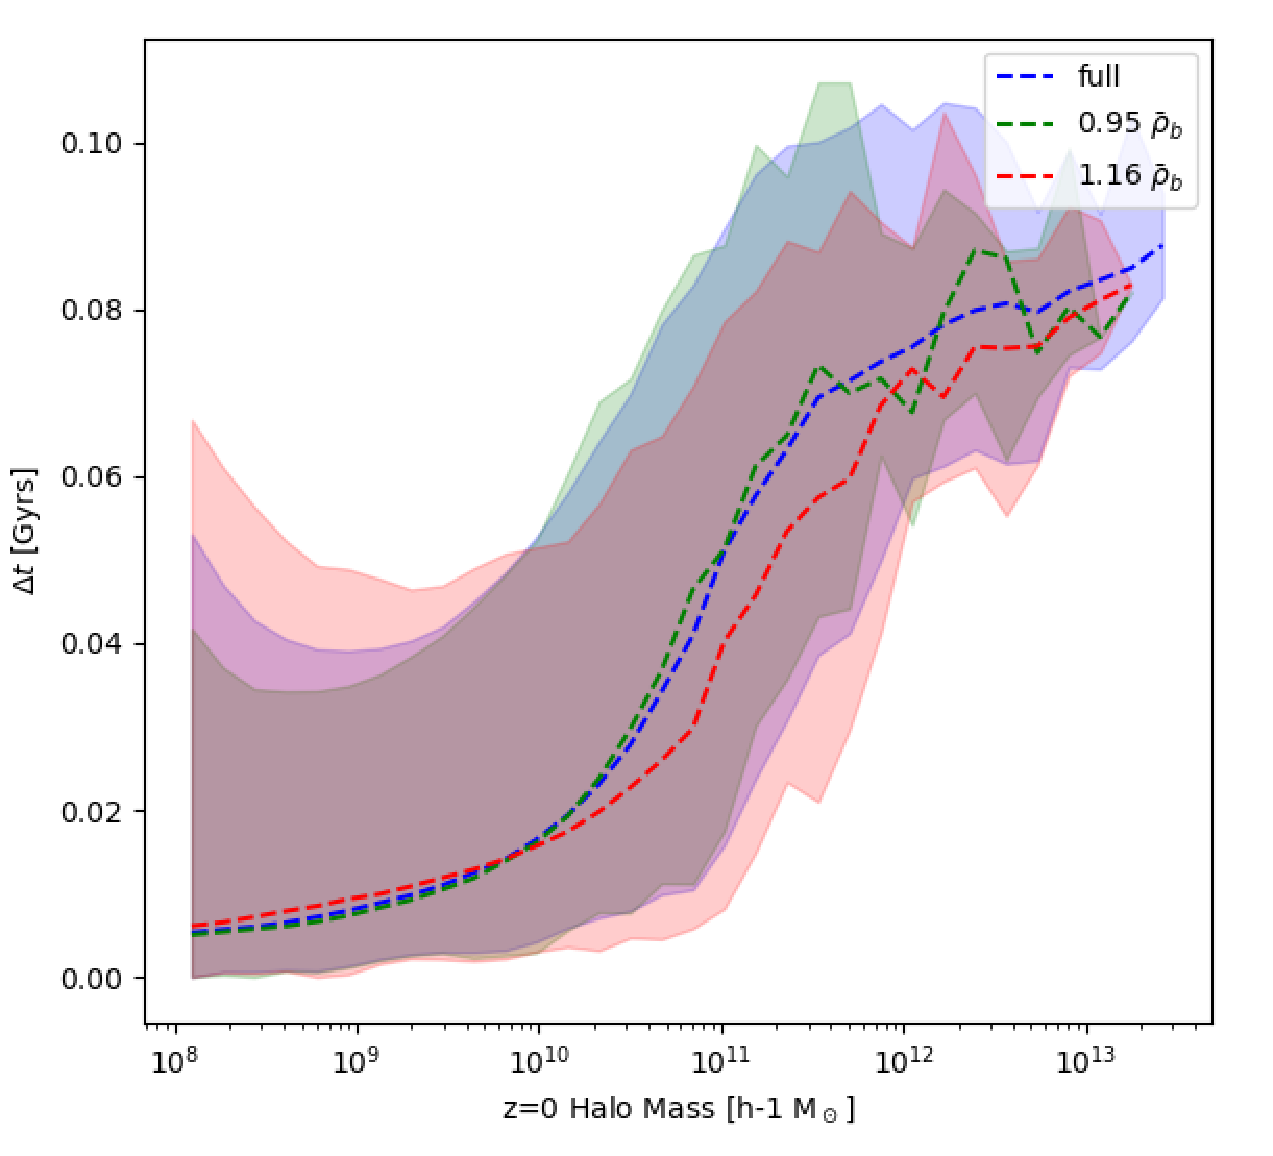
\includegraphics[width=.95\linewidth]{img/05/median_dt_envir.pdf}
%        \caption[Durée de réionisation et environnement]{Durée de réionisation en fonction de l'environnement.
%        Un environnement dense diminue la durée médiane d'ionisation des halos.
%		\label{fig:CODA_environnement}}
%\end{figure}


\subsection{Le cas du groupe local}

Les simulations présentées ici utilisent des conditions initiales disposant d'une paire de galaxies MW-M31 avec des caractéristiques proches de celles du Groupe Local  à $z=0$ (voir section \ref{sec:ICCODA}).
L'avantage de cette simulation est que le contexte cosmologique est suffisamment représentatif pour pouvoir déterminer si ce couple à été réionisé de manière autonome ou de manière externe, menant à des propriétés différentes.
Cette section est consacrée à l'étude de la réionisation de cette paire de galaxies particulières.

Ces galaxies sont représentées par les points sur la figure \ref{fig:CODA_t}. 
On y mesure qu'elles sont réionisées légèrement plus tard que la médiane de leur classe de masse mais toujours plus tôt que la moyenne du volume.
Dans le cas de la méthode des particules, les deux ont réionisées en même temps.
Cette méthode à tendance à considérer une grande partie de la masse provenant e l'\ac{IGM}, et étant donnée la proximité spatiale des progéniteur il est probable que leur environnement ait été ionisé en même temps.

Dans le cas de la méthode des progéniteurs, M31 a réionisée significativement plus tôt.
Ceci s'explique par le fait que M31 est plus massive que MW % et que son progéniteur le plus massif (celui qui est pris en compte avec cette méthode) l'est également.
et a donc formé des étoiles, et réionisé plus tôt que MW.


%Dans les deux cas la durée de réionisation de MW est plus courte que la médiane.

Les progéniteurs à redshift $z=10.8$ du couple Voie Lactée - Andromède sont superposés à la carte de redshift d'ionisation et représentés sur la figure \ref{fig:CODA_LG}.
On mesure que la dispersion spatiale de M31 est plus importante que celle de MW et le fait que M31 ait une durée de réionisation plus importante que MW est sans doute lié à cette étendue spatiale.
On remarque également que les progéniteurs ont tendance à être dans des bulles ionisées distinctes à redshift $z>10$, suggérant une réionisation autonome.
Dans le cas d'une réionisation par un front externe, un gradient de redshift serait présent sur la carte, ce qui n'est pas le cas ici.

\begin{figure}
		\centering
		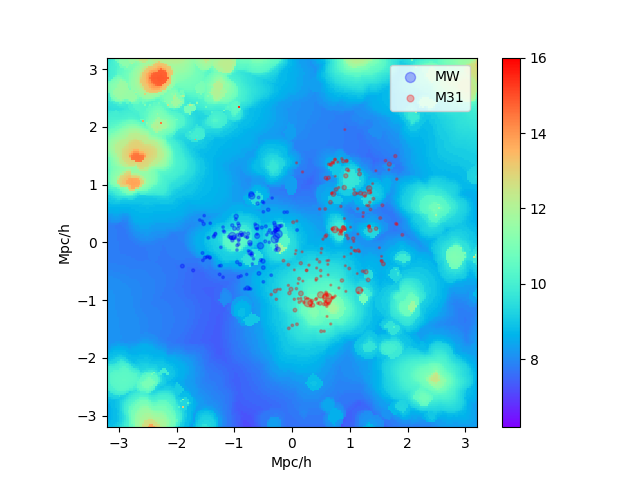
\includegraphics[width=.95\linewidth]{img/05/map_LG.png}
        \caption[Réionisation du groupe local]{Progéniteurs du couple M31-MW à redshift $z=10.8$ superposé à la carte de redshift d'ionisation.
		\label{fig:CODA_LG}}
\end{figure}


\subsection{Conclusions et perspectives}

%Cette étude utilise différentes méthodes mais la tendance générale reste la même.

Cette étude montre que les halos les plus massifs à $z=0$ réionisent plus tôt que les autres, car leurs sources de rayonnement ionisant apparaissent plus tôt et que leurs environnements sont généralement plus denses.
Ils ont également des durées de réionisations plus grandes.
Cette importante durée peut être expliquée par le fait que leur étendue spatiale et leur masse de gaz neutre soit plus importantes, mais aussi par le fait que la propagation de l'ionisation a tendance à être plus lente dans les environnements denses (voir conclusion de la section \ref{sec:intre:zreio}).
Les halos les plus massifs ont tendance à réioniser tôt mais lentement car ils se trouvent dans les régions denses et que les fronts ont des vitesses relativement faibles dans ces régions. %, puisque dans les régions les plus denses, les fronts d'ionisation ont des vitesses relativement faibles (la première phase de l'\ac{EoR}).
Quand le rayonnement atteint les zones de densités plus faible, les fronts d'ionisation accélèrent, et atteignent des halos qui seront réionisé plus tardivement mais de manière plus rapide expliquant le fait que les plus petits halos réionisent plus tard que la moyenne et extrêmement rapidement.
Cette interprétation mérite toutefois une analyse plus en détails.

L'application au groupe local tend à confirmer l'hypothèse que celui ci s'est réionisé de manière autonome et n'a pas été influencé par les grandes structures de son environnement comme Virgo.
%Comme mentionné par \, une réionisation interne a une incidence différente sur la distribution radiale des galaxies satellites qu'une réionisation externe.
Comme une réionisation interne a des conséquences sur la distribution radiale de galaxies satellites \citep{2011MNRAS.417L..93O}, une réionisation interne anisotrope pourrait avoir une influence sur la configuration des plans de satellites observés \citep{2015ApJ...800...34G}.
Par exemple une réionisation interne présentant une forte anisotropie il est possible que le rayonnement ait "éteint" une partie des satellites à haut redshift et dans une direction particulière, tandis qu'une autre partie aurait vu le rayonnement de manière plus tardive.
Potentiellement un tel scénario pourrait expliquer le plan de galaxies observé par \cite{2014Natur.511..563I}.